\UseRawInputEncoding
\documentclass[a4paper, 12pt, twoside]{article}

\usepackage[utf8]{inputenc}
\usepackage[T1]{fontenc}
\usepackage[french]{babel}
\usepackage{lmodern}
\usepackage[top=2.5cm, bottom=2cm, left=3cm, right=2.5cm, headheight=15pt]{geometry}
\usepackage{graphicx}
\usepackage{array}
\usepackage{hyperref}
\usepackage{listings}
\usepackage{xcolor}
%\usepackage{pagedegarde}
\lstdefinelanguage{javascript}{
  keywords={break, case, catch, continue, debugger, default, delete, do, else, finally, for, function, if, in, instanceof, new, return, switch, this, throw, try, typeof, var, void, while, with},
  keywordstyle=\color{blue}\bfseries,
  ndkeywords={class, export, boolean, throw, implements, import, this},
  ndkeywordstyle=\color{darkgray}\bfseries,
  identifierstyle=\color{black},
  sensitive=false,
  comment=[l]{//},
  morecomment=[s]{/*}{*/},
  commentstyle=\color{purple}\ttfamily,
  stringstyle=\color{red}\ttfamily,
  morestring=[b]',
  morestring=[b]"
}


\input{pagedegarde}

\title{KAMP : Application web de réseau social étudiant avec système de recommandation MBTI}
\entreprise{Université Paris Nanterre}
\datedebut{25/04/2026}
\datefin{24/05/2026}

\membrea{KESSILI EVA}
\membreb{AIT-ABAS YASMINE}
\membrec{TALBI MAISSA}
\membred{BOUZIDI SHAYMA}

\lstset{
    language=JavaScript,
    basicstyle=\ttfamily\small,
    keywordstyle=\color{blue},
    stringstyle=\color{red},
    commentstyle=\color{gray},
    breaklines=true,
    frame=single,
    numbers=left,
    numberstyle=\tiny,
    tabsize=2
}

\begin{document}

\pagedegarde

\section*{Remerciements}

Nous remercions notre enseignant pour son accompagnement durant ce projet informatique. 
Nous remercions également les membres du groupe pour leur implication dans la conception, le développement et les tests de l'application.

\newpage

\tableofcontents
\newpage

\section{Introduction}

Le projet KAMP consiste à développer une application web de réseau social destinée aux étudiants. 
L'objectif principal est de proposer une plateforme permettant aux utilisateurs de créer un profil, publier du contenu, communiquer avec d'autres étudiants et recevoir des recommandations de profils compatibles.

L'application s'inspire des réseaux sociaux modernes, mais elle ajoute une dimension originale grâce à un système de recommandation basé sur le profil MBTI des utilisateurs. 
Ce système permet de proposer des personnes potentiellement compatibles à partir du type de personnalité renseigné dans le profil.

Le projet a été développé avec React pour l'interface utilisateur et Firebase pour l'authentification et la gestion des données. 
Il comprend plusieurs fonctionnalités : inscription, connexion, création de profil, fil d'actualité, messages, notifications, commentaires, likes et recommandations MBTI.

\section{Environnement de travail}

Le projet a été réalisé dans un environnement de développement web moderne. 
Nous avons utilisé Visual Studio Code pour écrire et organiser le code source. 
Le projet a ensuite été sauvegardé et partagé grâce à GitHub.

L'application est une application web développée en JavaScript avec React. 
Elle fonctionne dans un navigateur web et utilise Firebase pour gérer les utilisateurs et les données.

Les principaux outils utilisés sont :

\begin{itemize}
    \item Visual Studio Code pour le développement ;
    \item GitHub pour le stockage et le partage du code ;
    \item React pour construire l'interface utilisateur ;
    \item Firebase Authentication pour l'inscription et la connexion ;
    \item Firestore Database pour stocker les messages, posts et notifications ;
    \item CSS pour la mise en forme de l'application.
\end{itemize}

\section{Description du projet et objectifs}

\subsection{Présentation générale}

KAMP est une application web de réseau social étudiant. 
Elle permet à un utilisateur de se connecter, de créer son profil et d'interagir avec d'autres utilisateurs à travers un fil d'actualité, un système de messages et des notifications.

L'application est organisée en plusieurs composants React. 
Chaque composant correspond à une partie précise de l'interface : authentification, profil, feed, messagerie, notifications, barre latérale, recommandations MBTI, etc.

\subsection{Objectifs du projet}

Les objectifs principaux du projet sont les suivants :

\begin{itemize}
    \item créer une application web interactive ;
    \item permettre l'inscription et la connexion des utilisateurs ;
    \item permettre la création d'un profil étudiant ;
    \item afficher un fil d'actualité avec des publications ;
    \item permettre aux utilisateurs de liker et commenter les publications ;
    \item créer une messagerie en temps réel ;
    \item afficher des notifications ;
    \item proposer un système de recommandation basé sur le MBTI ;
    \item obtenir une interface claire, moderne et simple à utiliser.
\end{itemize}

\section{Bibliothèques, outils et technologies}

Le projet utilise plusieurs bibliothèques et technologies.

\subsection{React}

React est utilisé pour construire l'interface utilisateur. 
L'application est divisée en composants indépendants, par exemple \texttt{Auth}, \texttt{Feed}, \texttt{Messages}, \texttt{Profile}, \texttt{PostCard} ou encore \texttt{AIMatchPage}.

React permet aussi de gérer les changements dynamiques dans l'application grâce aux hooks comme \texttt{useState}, \texttt{useEffect} et \texttt{useMemo}.

\subsection{Firebase}

Firebase est utilisé pour gérer la partie serveur du projet. 
Il permet de gérer l'authentification des utilisateurs et le stockage des données.

Dans le fichier \texttt{firebase.js}, l'application est connectée au projet Firebase avec le code suivant :

\begin{lstlisting}
import { initializeApp } from "firebase/app";
import { getAuth } from "firebase/auth";
import { getFirestore } from "firebase/firestore";

const app = initializeApp(firebaseConfig);

export const auth = getAuth(app);
export const db = getFirestore(app);
\end{lstlisting}

\subsection{Firebase Authentication}

Firebase Authentication est utilisé pour créer des comptes utilisateurs et permettre la connexion. 
Dans le composant \texttt{Auth.jsx}, les fonctions utilisées sont :

\begin{lstlisting}
createUserWithEmailAndPassword
signInWithEmailAndPassword
\end{lstlisting}

Ces fonctions permettent soit de créer un nouveau compte, soit de connecter un utilisateur existant.

\subsection{Firestore Database}

Firestore est utilisé pour stocker les données de l'application, notamment :

\begin{itemize}
    \item les publications ;
    \item les messages ;
    \item les notifications ;
    \item les commentaires ;
    \item les likes.
\end{itemize}

La fonction \texttt{onSnapshot} permet d'écouter les modifications en temps réel. 
Ainsi, lorsqu'un message ou une publication est ajouté, l'affichage peut se mettre à jour automatiquement.

\subsection{CSS}

Le fichier \texttt{App.css} permet de gérer l'apparence de l'application. 
Il définit le design général : barre latérale, cartes de publications, messages, profil, boutons, couleurs et mise en page.

\section{Travail réalisé}

\subsection{Authentification}

Nous avons réalisé un système d'inscription et de connexion grâce à Firebase Authentication.

Le composant \texttt{Auth.jsx} contient un formulaire permettant à l'utilisateur de saisir son adresse email et son mot de passe. 
Selon le mode choisi, l'utilisateur peut soit se connecter, soit créer un nouveau compte.

\begin{lstlisting}
await signInWithEmailAndPassword(auth, email, password);

await createUserWithEmailAndPassword(auth, email, password);
\end{lstlisting}

Cette fonctionnalité est essentielle car elle permet de sécuriser l'accès à l'application.

\subsection{Création du profil utilisateur}

Après la connexion, l'utilisateur doit créer son profil. 
Le composant \texttt{SetupProfile.jsx} permet de renseigner :

\begin{itemize}
    \item un prénom ;
    \item un type MBTI ;
    \item une licence ou formation ;
    \item une photo de profil.
\end{itemize}

Les données du profil sont sauvegardées dans le \texttt{localStorage}. 
Cela permet de conserver les informations même après un rechargement de la page.

\begin{lstlisting}
localStorage.setItem(
  "kamp-profile",
  JSON.stringify(profile)
);
\end{lstlisting}

\subsection{Fil d'actualité}

Le composant \texttt{Feed.jsx} permet d'afficher les publications des utilisateurs. 
Les publications sont récupérées depuis Firestore grâce à \texttt{onSnapshot}.

\begin{lstlisting}
const unsubscribe = onSnapshot(
  collection(db, "posts"),
  (snapshot) => {
    const loadedPosts = snapshot.docs.map((doc) => ({
      id: doc.id,
      ...doc.data()
    }));

    setPosts(loadedPosts.reverse());
  }
);
\end{lstlisting}

L'utilisateur peut publier un message dans le feed. 
Chaque publication contient le nom de l'utilisateur, son MBTI, sa formation, son texte, son image éventuelle, ses likes et ses commentaires.

\subsection{Likes et commentaires}

Le composant \texttt{PostCard.jsx} gère l'affichage d'une publication. 
Il permet à l'utilisateur de liker un post et d'ajouter un commentaire.

Pour les likes, nous utilisons la fonction \texttt{increment} de Firebase :

\begin{lstlisting}
await updateDoc(
  doc(db, "posts", post.id),
  {
    likes: increment(1)
  }
);
\end{lstlisting}

Pour les commentaires, nous utilisons \texttt{arrayUnion}, qui permet d'ajouter un commentaire à la liste des commentaires déjà présents.

\begin{lstlisting}
await updateDoc(
  doc(db, "posts", post.id),
  {
    comments: arrayUnion(newComment)
  }
);
\end{lstlisting}

\subsection{Notifications}

Le composant \texttt{Notifications.jsx} affiche les notifications enregistrées dans Firestore. 
Une notification est créée lorsqu'un utilisateur aime ou commente une publication.

Exemple de création d'une notification :

\begin{lstlisting}
await addDoc(collection(db, "notifications"), {
  from: profile.username,
  text: "a aimé ton post",
  createdAt: serverTimestamp()
});
\end{lstlisting}

Cette fonctionnalité permet de rendre l'application plus interactive.

\subsection{Messagerie}

Le composant \texttt{Messages.jsx} permet de créer une messagerie avec plusieurs salons :

\begin{itemize}
    \item Général ;
    \item Révisions ;
    \item Gaming ;
    \item Vocal nuit.
\end{itemize}

Les messages sont stockés dans Firestore dans une collection correspondant au salon choisi.

\begin{lstlisting}
collection(db, "rooms", currentRoom, "messages")
\end{lstlisting}

La fonction \texttt{onSnapshot} permet d'afficher les messages en temps réel.

\subsection{Recommandation MBTI}

Le système de recommandation est une partie importante du projet. 
Il est présent dans les composants \texttt{AIMatch.jsx} et \texttt{AIMatchPage.jsx}.

L'utilisateur renseigne son type MBTI lors de la création de son profil. 
Ensuite, l'application utilise un tableau de correspondances pour proposer des profils compatibles.

Exemple :

\begin{lstlisting}
INTJ: [
  {
    name: "Emma",
    mbti: "ENFP",
    compatibility: 92
  },
  {
    name: "Nathan",
    mbti: "ENTP",
    compatibility: 88
  }
]
\end{lstlisting}

Le programme récupère le MBTI de l'utilisateur avec :

\begin{lstlisting}
profile?.mbti?.toUpperCase()
\end{lstlisting}

Puis il affiche les profils recommandés avec leur pourcentage de compatibilité.

Cette fonctionnalité montre que l'application ne se limite pas à un réseau social classique. 
Elle propose aussi une recommandation personnalisée selon le profil de l'utilisateur.

\subsection{Interface utilisateur}

L'interface est organisée autour d'une barre latérale qui permet de naviguer entre les différentes pages :

\begin{itemize}
    \item Feed ;
    \item Messages ;
    \item Notifications ;
    \item IA Match ;
    \item Déconnexion.
\end{itemize}

Le composant \texttt{Sidebar.jsx} permet cette navigation.

\section{Difficultés rencontrées}

Plusieurs difficultés ont été rencontrées pendant le projet.

La première difficulté a été la compréhension de Firebase. 
Il fallait comprendre comment connecter l'application à Firebase, comment utiliser l'authentification et comment stocker des données dans Firestore.

La deuxième difficulté a été la gestion des états avec React. 
L'application utilise plusieurs états pour stocker les messages, les posts, les profils, les commentaires ou encore la page actuellement affichée.

Une autre difficulté a été la messagerie en temps réel. 
Il fallait faire en sorte que les messages apparaissent automatiquement sans recharger la page.

Enfin, l'organisation du code a également demandé du travail. 
Comme l'application contient plusieurs composants, il fallait bien séparer les fichiers pour rendre le projet plus clair.

\begin{lstlisting}
REPARTITION DU TRAVAIL :
- Yasmine : 15%
- Eva : 30%
- Shayma : 30%
- Maissa : 25%

\end{lstlisting}

\section{Bilan}

\subsection{Conclusion}

Ce projet nous a permis de développer une application web complète avec React et Firebase. 
Nous avons appris à construire une interface avec plusieurs composants, à gérer l'authentification des utilisateurs et à manipuler une base de données en temps réel.

L'application KAMP possède plusieurs fonctionnalités importantes : connexion, profil, publications, likes, commentaires, notifications, messagerie et recommandations MBTI. 
Le projet répond donc aux objectifs fixés au départ.

\subsection{Perspectives}

Plusieurs améliorations pourraient être ajoutées à l'application :

\begin{itemize}
    \item améliorer le système de recommandation avec un algorithme plus avancé ;
    \item stocker les profils directement dans Firestore au lieu du localStorage ;
    \item ajouter une vraie page de modification du profil ;
    \item améliorer la sécurité des règles Firebase ;
    \item rendre l'application entièrement responsive pour mobile ;
    \item ajouter un système de recherche d'utilisateurs ;
    \item ajouter des images stockées dans Firebase Storage.
\end{itemize}

\newpage

\section{Bibliographie}

\renewcommand{\bibname}{}
\renewcommand{\refname}{}

\begin{thebibliography}{2}

\bibitem[REACT]{react}
React, Documentation officielle, Meta.

\bibitem[FIREBASE]{firebase}
Firebase, Documentation officielle, Google.

\end{thebibliography}

\newpage

\section{Webographie}

\begin{thebibliography}{3}

\bibitem[REACTWEB]{reactweb}
\url{https://react.dev/}

\bibitem[FIREBASEWEB]{firebaseweb}
\url{https://firebase.google.com/}

\bibitem[GITHUB]{github}
\url{https://github.com/}

\end{thebibliography}

\newpage

\section{Annexes}

\appendix

\makeatletter
\def\@seccntformat#1{Annexe~\csname the#1\endcsname:\quad}
\makeatother

\section{Cahier des charges}

Le cahier des charges du projet était de créer une application web fonctionnelle autour d'un réseau social étudiant.

Les fonctionnalités prévues étaient :

\begin{itemize}
    \item inscription et connexion ;
    \item création d'un profil utilisateur ;
    \item publication de messages ;
    \item affichage d'un fil d'actualité ;
    \item likes et commentaires ;
    \item notifications ;
    \item messagerie ;
    \item recommandations de profils compatibles.
\end{itemize}

Les fonctionnalités réalisées sont :

\begin{itemize}
    \item inscription et connexion avec Firebase ;
    \item création de profil avec nom, MBTI, formation et photo ;
    \item feed de publications ;
    \item likes ;
    \item commentaires ;
    \item notifications ;
    \item messagerie en temps réel ;
    \item recommandations MBTI ;
    \item interface avec barre latérale.
\end{itemize}

\section{Exemple d'exécution du projet}

Pour montrer le fonctionnement de l'application, il est possible d'ajouter ici des captures d'écran :

\begin{itemize}
    \item page de connexion ;
    \item page de création de profil ;
    \item fil d'actualité ;
    \item publication d'un post ;
    \item ajout d'un commentaire ;
    \item réception d'une notification ;
    \item affichage des recommandations MBTI ;
    \item messagerie.
\end{itemize}

Exemple de scénario d'utilisation :

\begin{figure}
    \centering
    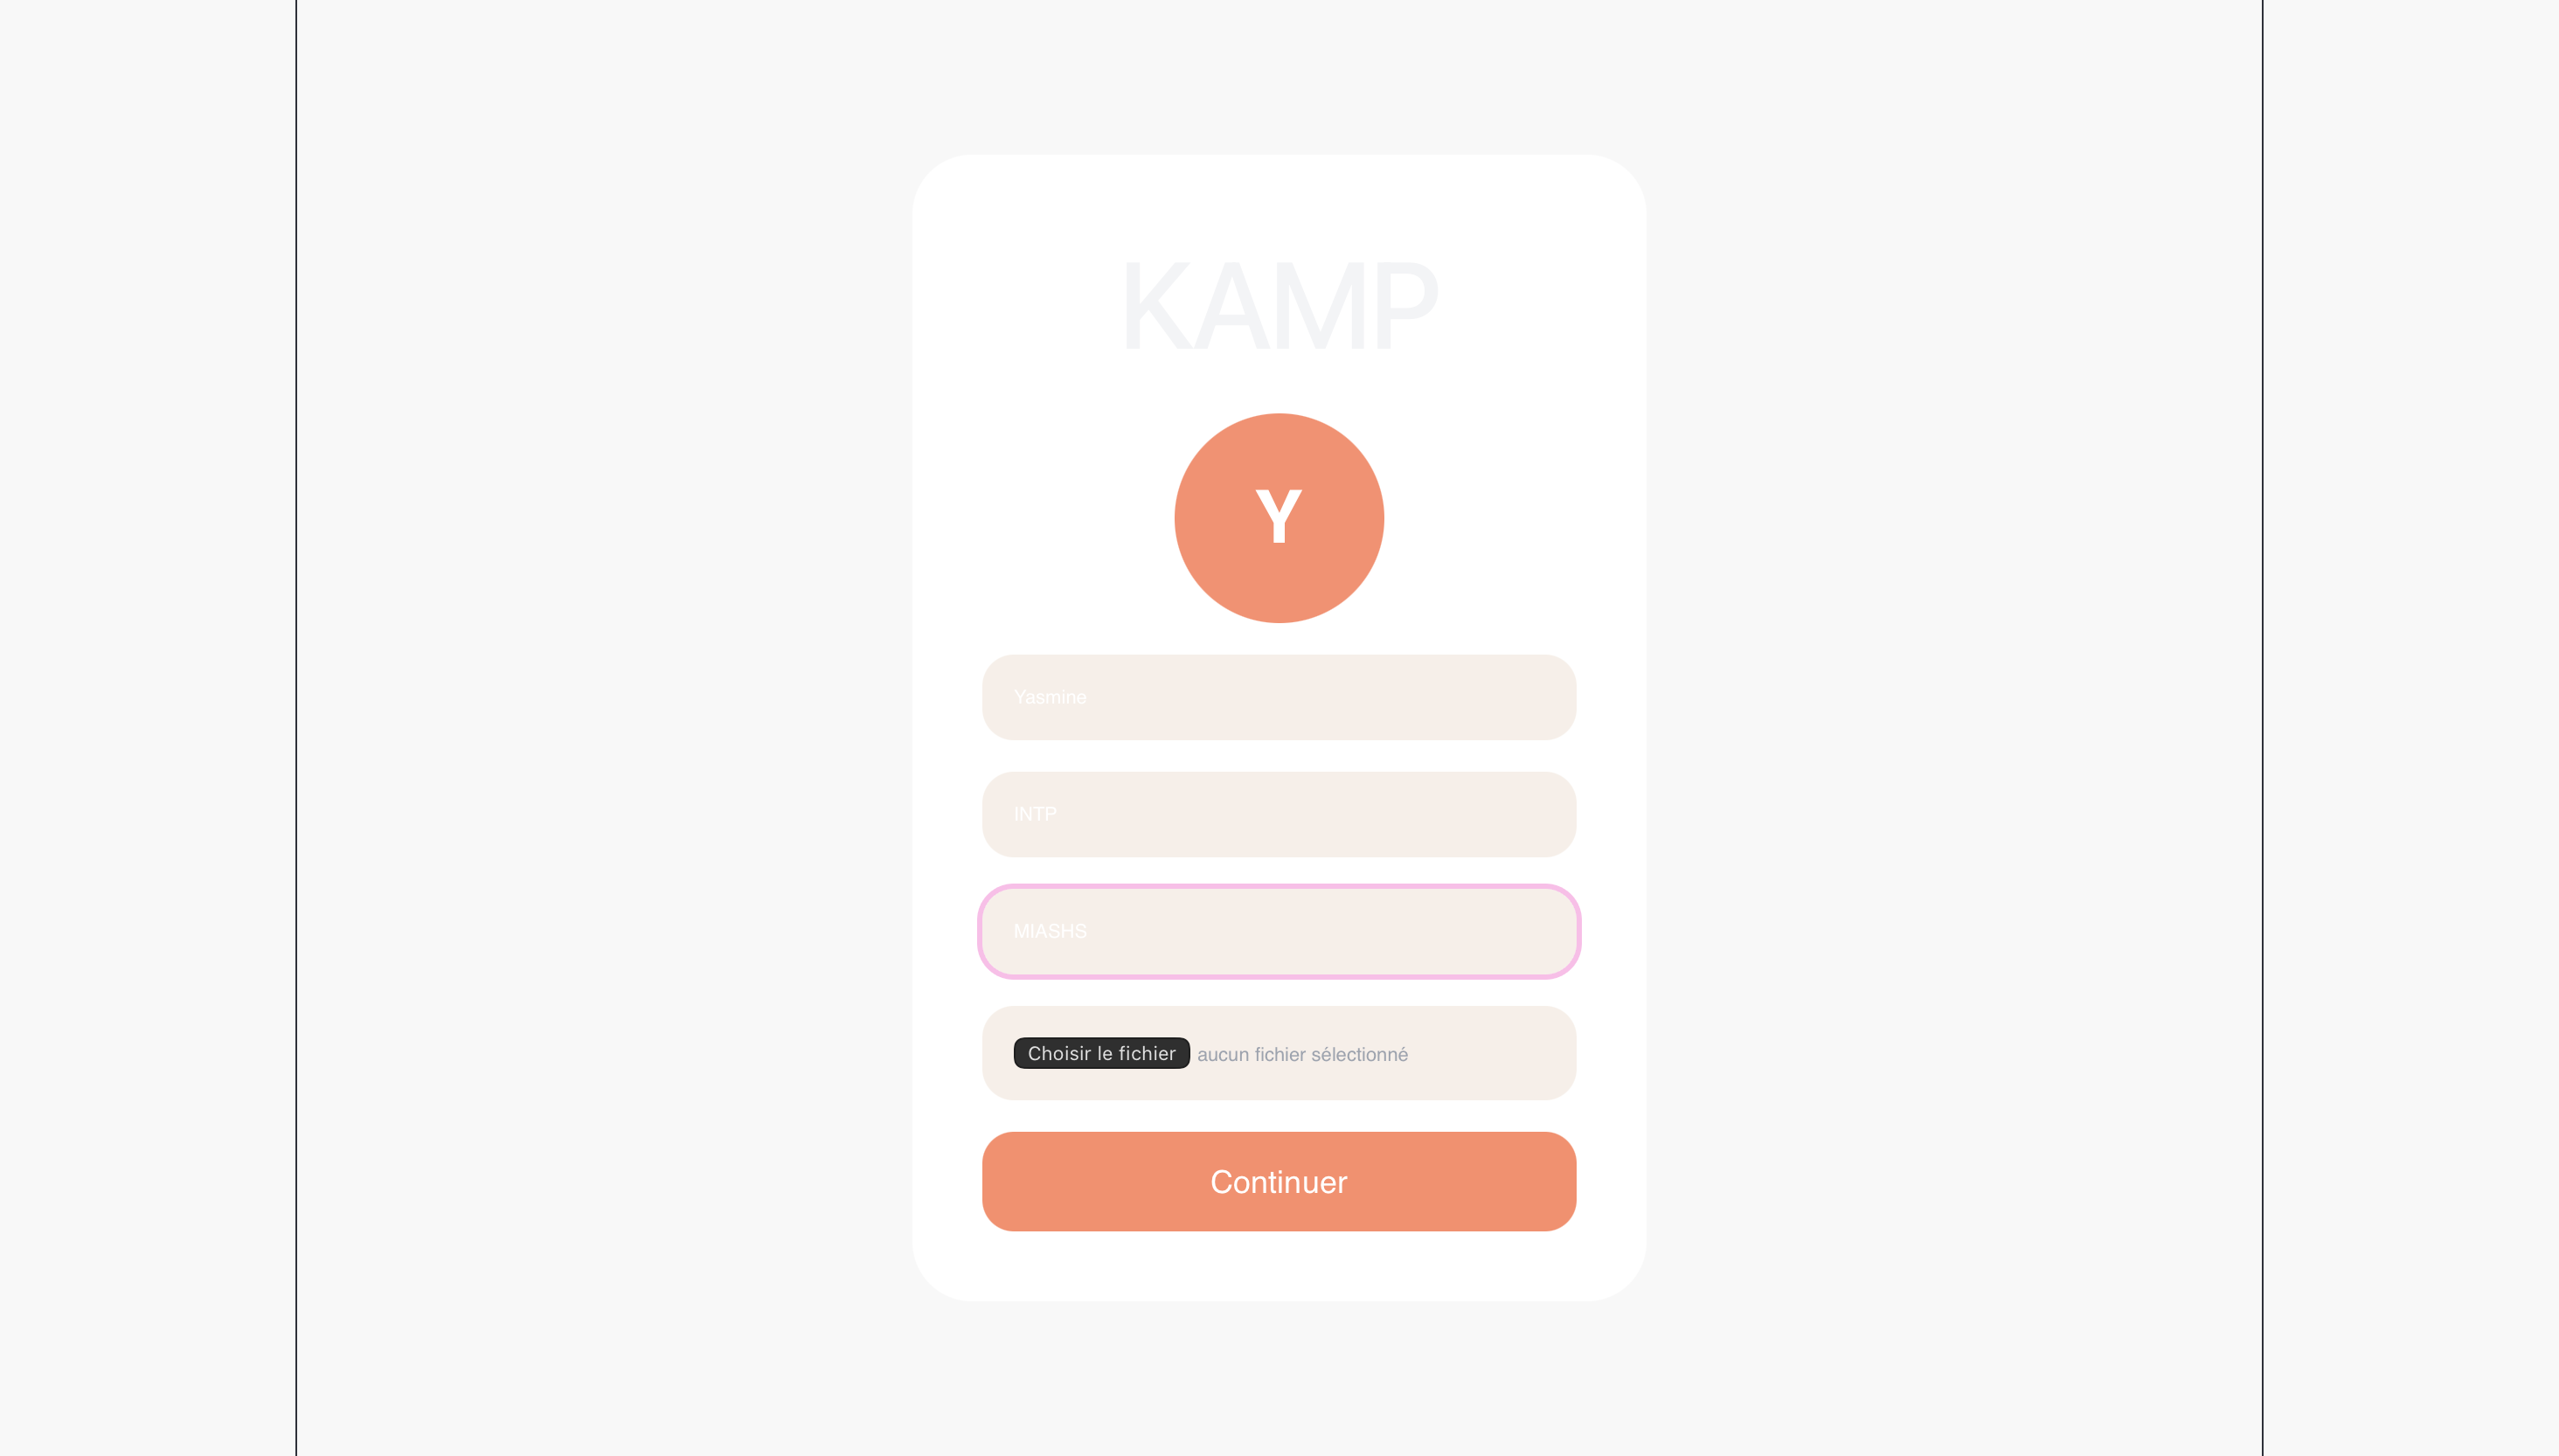
\includegraphics[width=0.5\linewidth]{Capture d’écran 2026-05-24 à 03.49.50.png}
    \caption{Page de connexion}
    \label{fig:placeholder}
\end{figure}
\begin{figure}
    \centering
    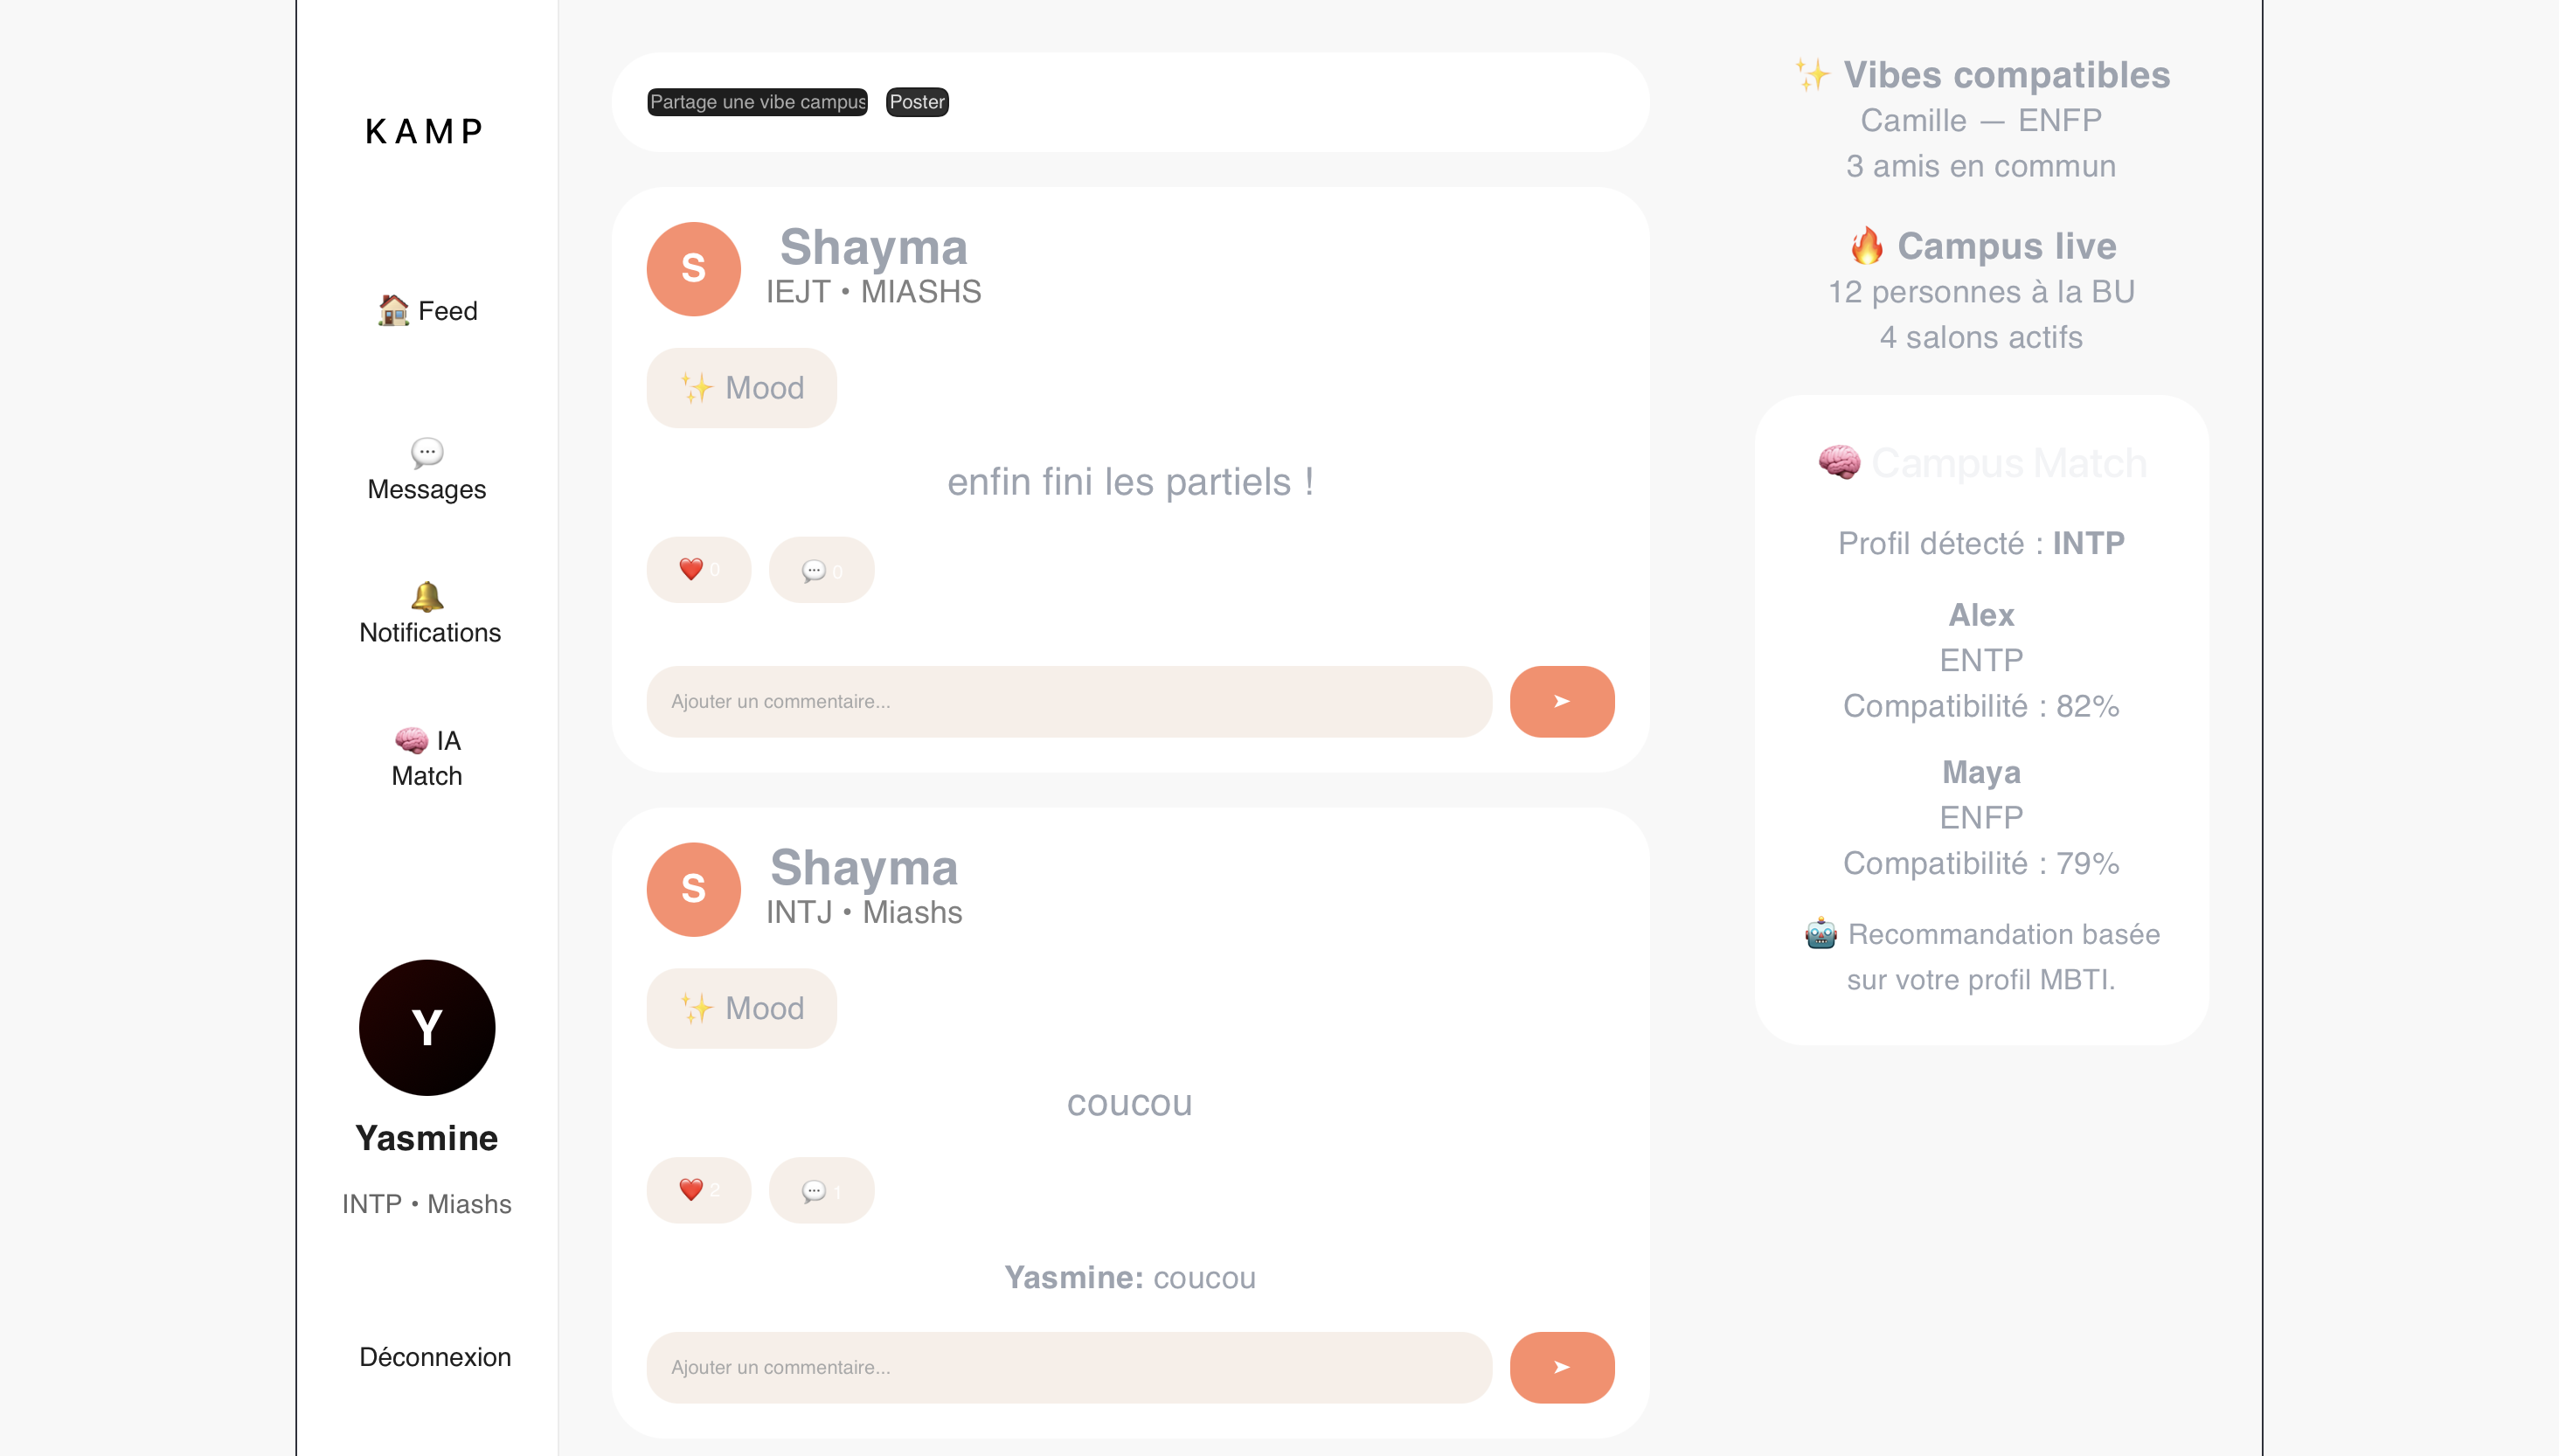
\includegraphics[width=0.5\linewidth]{Capture d’écran 2026-05-24 à 03.37.53.png}
    \caption{Feed de l'application}
    \label{fig:placeholder}
\end{figure}
\begin{figure}
    \centering
    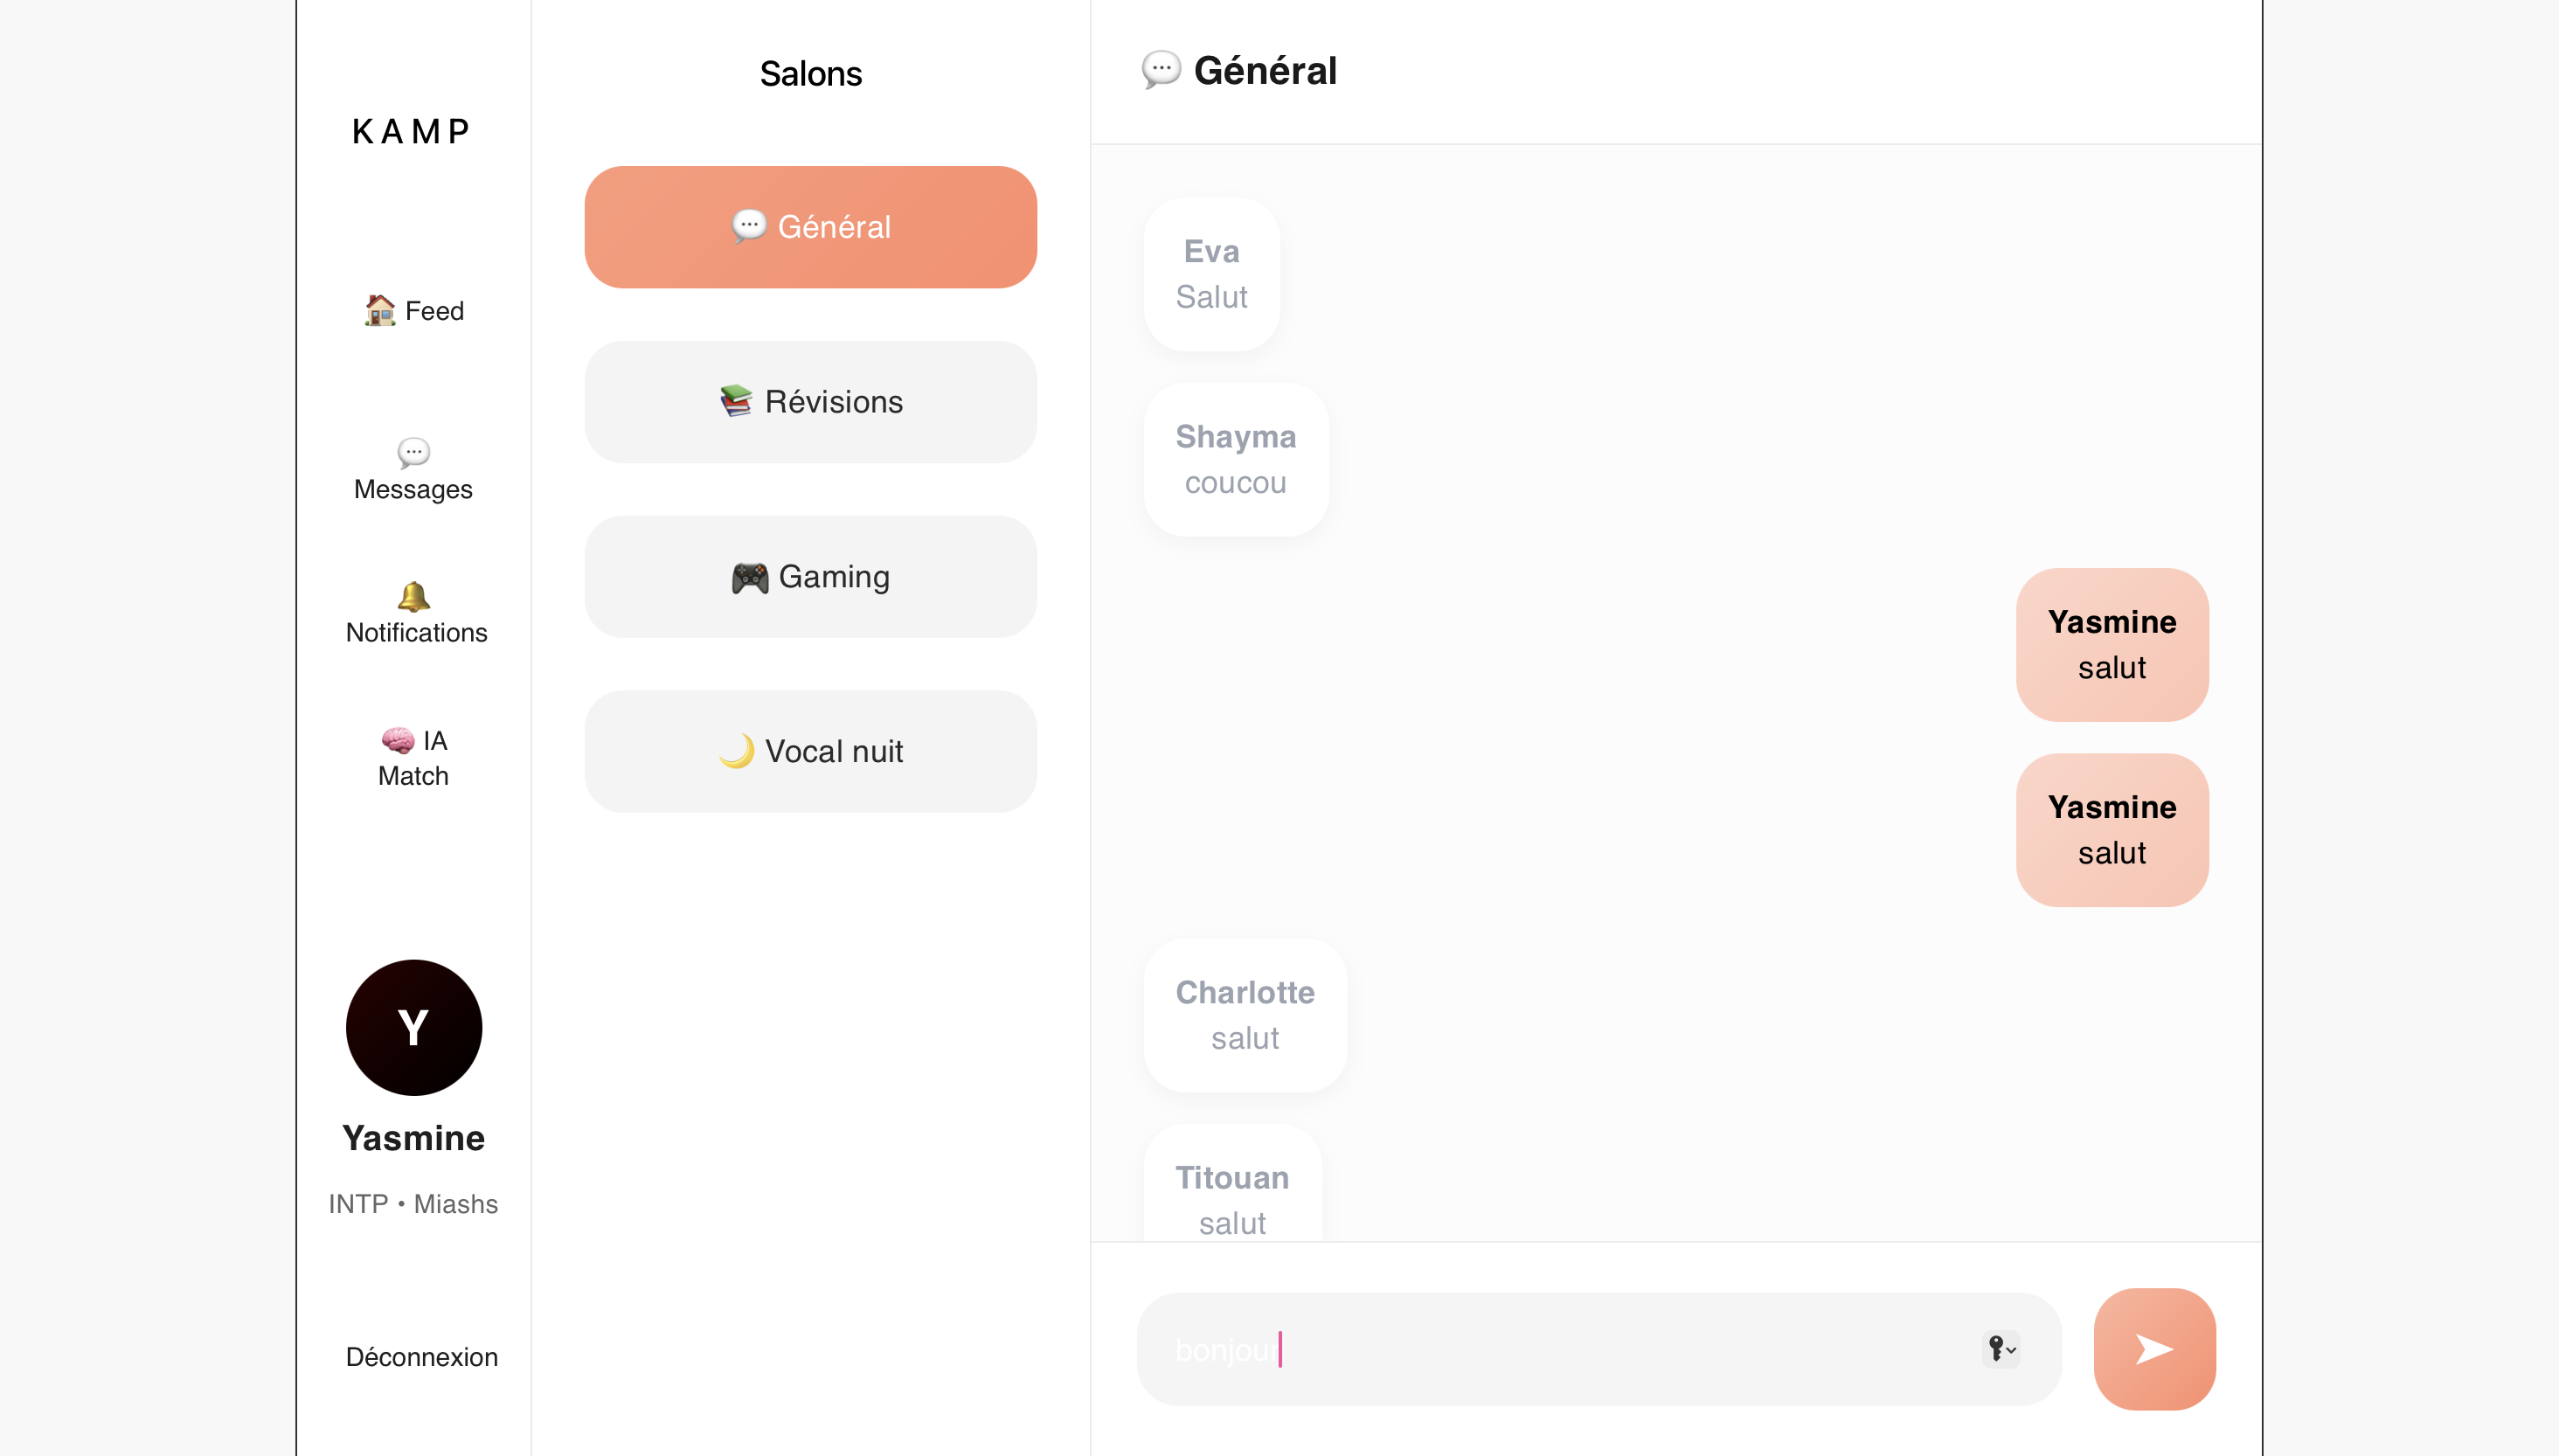
\includegraphics[width=0.5\linewidth]{Capture d’écran 2026-05-24 à 03.44.44.png}
    \caption{Salons de discussions}
    \label{fig:placeholder}
\end{figure}
\begin{figure}
    \centering
    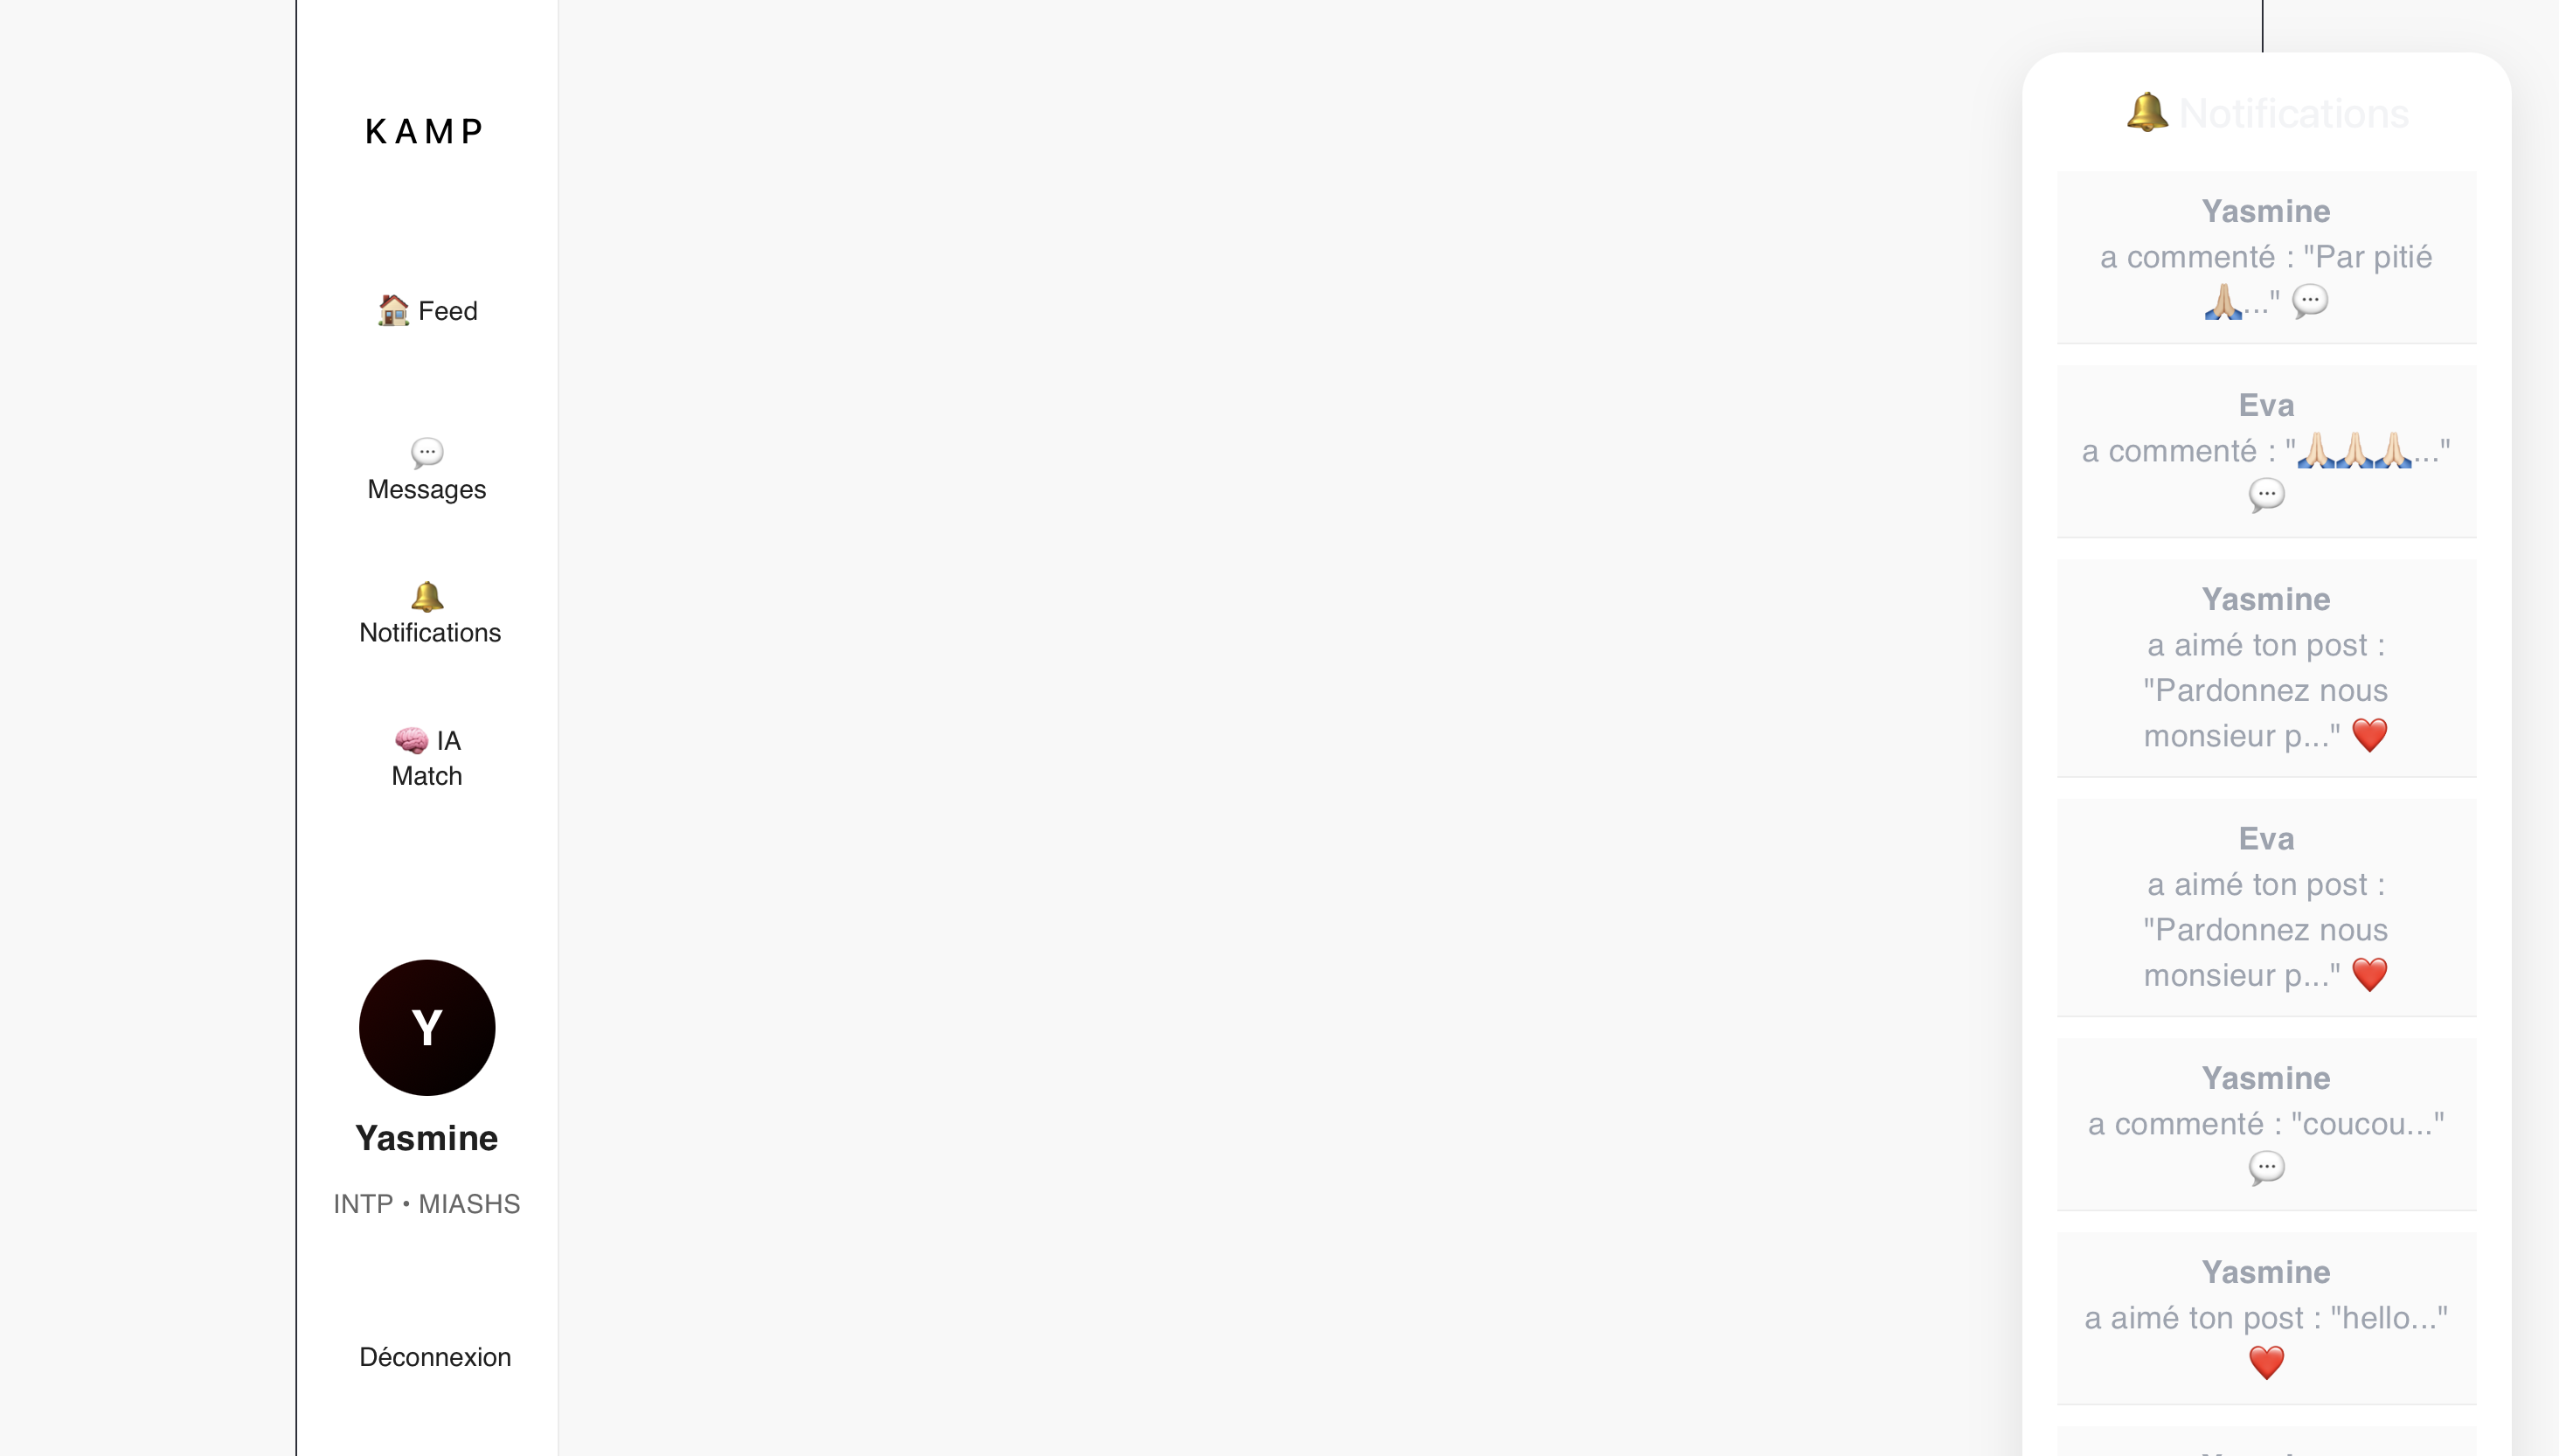
\includegraphics[width=0.5\linewidth]{Capture d’écran 2026-05-24 à 03.55.02.png}
    \caption{Page des notifications}
    \label{fig:placeholder}
\end{figure}
\begin{enumerate}
    \item L'utilisateur ouvre l'application KAMP.
    \item Il crée un compte avec une adresse email et un mot de passe.
    \item Il complète son profil avec son prénom, son MBTI et sa formation.
    \item Il accède au feed.
    \item Il publie un message.
    \item Un autre utilisateur peut liker ou commenter la publication.
    \item Une notification est créée.
    \item L'utilisateur peut consulter la page IA Match pour voir des profils compatibles.
    \item Il peut aussi envoyer des messages dans les salons de discussion.
\end{enumerate}

\section{Manuel utilisateur}

Pour utiliser l'application, l'utilisateur doit d'abord se créer un compte ou se connecter à un compte existant.

Après la connexion, il doit compléter son profil en indiquant son prénom, son type MBTI, sa formation et éventuellement une photo.

Une fois le profil créé, l'utilisateur arrive sur le fil d'actualité. 
Il peut publier un message, consulter les publications des autres utilisateurs, liker et commenter.

La barre latérale permet de naviguer dans l'application :

\begin{itemize}
    \item le bouton Feed permet de revenir au fil d'actualité ;
    \item le bouton Messages permet d'accéder aux salons de discussion ;
    \item le bouton Notifications permet d'afficher les notifications ;
    \item le bouton IA Match permet de voir les profils compatibles ;
    \item le bouton Déconnexion permet de quitter le compte.
\end{itemize}

\end{document}